\documentclass[
  ngerman,
  DIV=14
]{scrartcl}
\usepackage{babel}
\usepackage{csquotes}

% typography
\usepackage{fontspec}
%\usepackage[utopia]{mathdesign}
\usepackage{newpxmath}
\setsansfont{Open Sans}[
  BoldFont={Open Sans Bold},
  ItalicFont={Open Sans Italic}]
\setmonofont[Scale=0.87]{Menlo}
\setmainfont{Palatino}
\linespread{1.15}
%\renewcommand\familydefault{\sfdefault}
\usepackage[factor=1000]{microtype}

% graphics, drawings, etc.
\usepackage{xcolor}
\usepackage{graphicx}
\usepackage{pgfplots}
\usepackage{tikz}
\usepackage{soul}
\usetikzlibrary{shapes.geometric}
\usetikzlibrary{shapes.arrows}
\usetikzlibrary{positioning}
\usetikzlibrary{pgfplots.polar}

% highlighting, lists, code
\usepackage{listings}
\lstset{
  basicstyle=\ttfamily,
  numberstyle=\sffamily\footnotesize\color{gray},
  %escapeinside=||,
  keywordstyle=\color{blue!50!black},
  stringstyle=\color{green!50!black}}

% math
\usepackage{amsmath}
\usepackage{siunitx}

% links
\usepackage[
  colorlinks,
  linkcolor={red!50!black},
  citecolor={blue!50!black},
  urlcolor={blue!80!black}
]{hyperref}

\subject{Visual Computing}
\title{Fouriertheorie}
\subtitle{Übungsblatt 4}
\author{Patrick Elsen, Dmytro Klepatskyi,\\Costa Weiland, Nana Atchoukeu Chris-Mozart}
\date{Wintersemester 2018-2019}
\publishers{Technische Universität Darmstadt}

\begin{document}
\maketitle

\section*{Aufgabe 1: Abtastung}

\emph{Die Signale $f_1(t)$ und $f_2(t)$ werden mit den Abtastzeiten $T_1 = 1/400s$ und $T_2 = 1/1500s$ abgetastet.}
\begin{align*}
f_1(t) &= \sin(2 * \pi * 100) = 0\\
f_2(t) &= \sin(4000 * \pi) = 0 
\end{align*}

\emph{Wird das Abtasttheorem eingehalten?}

Ja, auf jeden Fall: sowohl $f_1$ als auch $f_2$ sind konstante Ausdrücke, die nicht von $t$ abhängen.

Anders würde es aussehen, wenn es sich hierbei um einen Tippfehler handelt, und $f_1(t) = \sin(2 * \pi * 100 * t)$ sowie $f_2(t) = \sin(4000 * \pi * t)$ gemeint sind. Das könnte eigentlich garnicht sein, da das Übungsblatt nicht korrigiert wurde. Aber dennoch gehen wir davon aus. Laut dem Abtasttheorem von Whittaker-Shannon wissen wir, dass für eine Funktion $f(t)$ mit der endlichen Grenzfrequenz $u_G$ wir eine Abtastfrequenz nehmen müssen, die mindestens doppelt so hoch ist wie $u_G$. Die Funktion $f_1$ ist eine pure Sinusfunktion mit einer Frequenz von 100 Hz, eine Abtastrate von $T_1 = 1/400s$ ist also akzeptabel, hier ist das Abtasttheorem eingehalten. Anders sieht es bei der $f_2$ aus, diese hat eine Frequenz von 2000 Hz, die Abtastrate $T_2 = 1/1500s$ ist hier nicht ausreichend um das Abtasttheorem zu erfüllen. 

\emph{Welchen Effekt erwarten Sie, wenn das Abtasttheorem nicht eingehalten ist? Erklären Sie diesen kurz.}

Wenn ein Signal mit einer zu niedrigen Frequenz abgetastet wird, dann wird es nicht korrekt aufgezeichnet und kann nicht richtig rekonstruiert werden. Es entsteht ein sogenanntes Aliasing.

\section*{Aufgabe 2: Faltung}

\emph{Was besagt der Faltungssatz? Nennen Sie eine in der Vorlesung genannte Anwendung und erklären Sie, warum der Faltungssatz angewandt wird.}

Der Faltungssatz besagt: \enquote{Einer Faltung im Ortsraum entspricht einer Multiplikation im Frequenzraum}. Eine Faltung ist eine Operation, die man auf zwei Funktionen anwenden kann. Hierbei wird eine Funktion an der y-Achse gespiegelt, an der x-Achse verschoben, die Funktionen werden multipliziert und integriert. Diese Operation entspricht einer Multiplikation dieser Funktionen im Frequenzraum. Damit werden unter anderen Filter realisiert.

\section*{Aufgabe 3: Fouriertheorie}

\emph{Die Fourierreihe ist definiert durch}
\begin{align*}
  f(x) = \sum_{n=0}^{\infty} (a_n \cos(n x) + b_n \sin(n x))
\end{align*}

\emph{mit}
\begin{align*}
a_0 = \frac{1}{2n}\int_{-\pi}^{\pi} f(x) dx  
\end{align*}

\emph{Gegeben ist die folgende 2π-periodische Rechteckfunktion}
\begin{align*}
f(x) = \begin{cases}
  -1, & \text{wenn } -\pi \leq x < -\frac{\pi}{2}\\
  0, & \text{wenn } -\frac{\pi}{2} \leq x < \frac{\pi}{2}\\
  1, & \text{wenn } \frac{\pi}{2} \leq x < \pi
\end{cases} 
\end{align*}


\emph{Berechnen Sie die Fourierkoeffizienten und geben Sie die so weit wie möglich vereinfachte resultierende Fourierreihe an. Geben Sie auch alle Zwischenschritte an.}

\begin{align*}
a_n 
  &= \frac{1}{\mathrm\pi}
  \int_{-\pi}^\pi f(x)\cos(n x) dx\\
  &= \frac{1}{\mathrm\pi} \left[\int_{-\pi}^{-\frac{\pi}{2}} (-1) \cos(n x) dx + \int_{-\frac{\pi}{2}}^\frac{\pi}{2} (0) \cos(n x) dx + \int_\frac{\pi}{2}^\pi (-1) \cos(n x) dx\right]\\
&=\frac{1}{\pi}\left[-\left(\frac{\sin(-\frac{\mathrm{πn}}2)}n-\frac{\sin(-\mathrm{πn})}n\right)+0-\left(\frac{\sin(\mathrm{πn})}n-\frac{\sin(\frac{\mathrm{πn}}2)}n\right)\right]\\
&=-\frac1{\mathrm\pi}\left(-\frac{\sin(\frac{\mathrm{πn}}2)}n-\frac{\sin(\frac{\mathrm{πn}}2)}n\right)\\
&=-\frac{1}{\pi}\left(-2\frac{\sin(\frac{\mathrm\pi}2n)}{\displaystyle n}\right)=\frac2{\mathrm\pi}\frac{\sin(\frac{\mathrm\pi}{2} n)}{n}
\end{align*}
\begin{align*}
b_n 
&= \frac{1}{\pi} \int_{-\pi}^\pi f(x) \sin(n x) dx\\
& =\frac{1}{\pi} \left[\int_{-\pi}^{-\frac{\pi}{2}}(-1)\sin(n x) dx + \int_{-\frac{\pi}2}^\frac{\mathrm\pi}2(0)\;\sin(nx)dx\;+\int_\frac{\pi}{2}^\pi(-1)\sin(n x) dx\right]\\
&=\frac{1}{\pi}\left[\left(\frac{\cos(-\frac{\pi n}2)}n-\frac{\cos(-\pi n)}n\right)+0+\left(\frac{\cos(\pi n)}n-\frac{\cos(\frac{\pi n}{2})}n\right)\right]=\\
&=\frac{1}{\pi}\left(\frac{\cos(\frac{\pi n}2)}n-\frac{\cos(\pi n)}n+\frac{\cos(\pi n)}n-\frac{\cos(\frac{\pi n}2)}n\right)\\
&=\frac{1}{\pi}0\\
&=0
\end{align*}
\begin{align*}
f(x)
&= \frac{2}{\mathrm\pi}{\sum_{n=0}^\infty}\frac{\sin({\frac{\mathrm\pi}2}n)\cos(nx)}n\\
&=\frac2{\pi}\left(\frac{\sin({\frac{\pi}2})\cos(x)}1+\frac{\sin(\mathrm\pi)\cos(2x)}2+\frac{\sin({\frac{3\mathrm\pi}2})\cos(3x)}3+...\right)\\
&=\frac2{\pi}\left(\cos(x)-\frac{\cos(3x)}3+\frac{\cos(5x)}5-\frac{\cos(7x)}7+...\right)
\end{align*}


\section*{Aufgabe 4: Mathematische Grundlagen}

\emph{Tragen Sie die folgenden Punkte}
\begin{align*}
A &= (5, 7) \quad A \in (\mathbb{R} \times \mathbb{R})\\
B &= (5, \frac{\pi}{2}) \quad B \in (\mathbb{R} \times [0, 2\pi])
\end{align*}

\emph{in jeweils ein passendes Koordinatensystem ein und transformieren sie Polarkoordinaten zu kartesischen Koordinaten und umgekehrt. Runden Sie auf 4 Nachkommastellen.}


Um $A$, welches in einem kartesischen Koordinatensystem angegeben ist, in ein polares Koordinatensystem umzuformen, rechnen wir:
\begin{align*}
  r &= \sqrt{x^2 + y^2} = \sqrt{25 + 49} = 8,6023\\
  \varphi &= \arctan(\frac{7}{5}) = 0,9505
\end{align*}

Um $B$, welches in einem polaren Koodinatensystem angegeben ist, in ein karteisches System umzuwandeln, rechnen wir:
\begin{align*}
  x &= r \cos(\varphi) = 5 \cdot 0 = 0\\
  y &= r \sin(\varphi) = 5 \cdot 1 = 5\\
\end{align*}

Jetzt können wir die beiden Punkte in Koordinatensysteme zeichnen.

\begin{tikzpicture}
\begin{axis}[xmin=0,ymin=0,xmax=10,ymax=10]
\addplot[mark=*] coordinates {(5,7)} node[label={$A$}] {};
\end{axis}
\end{tikzpicture}

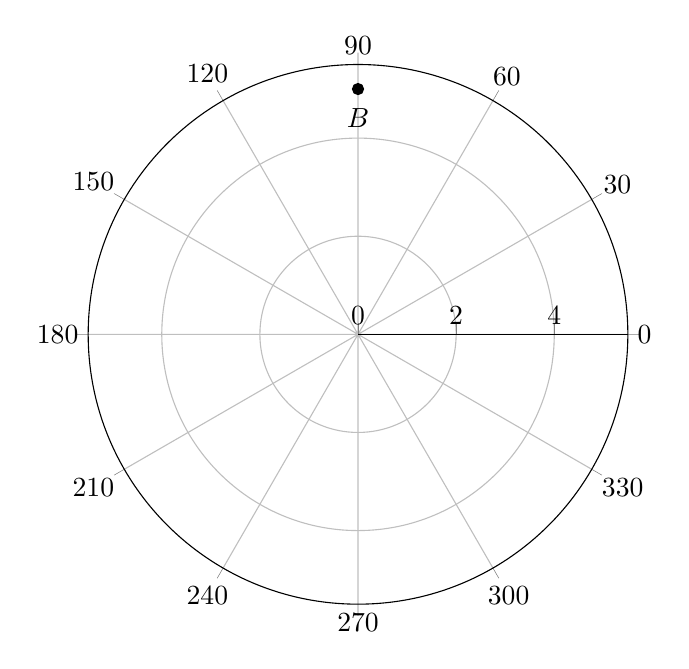
\begin{tikzpicture}
\begin{polaraxis}
\addplot[mark=*] coordinates {(90,5)} node[label=below:{$B$}] {};
\end{polaraxis}
\end{tikzpicture}


\emph{Gegeben seien die folgenden Vektoren:}
\begin{align*}
\vec{a} &= \begin{pmatrix}3\\0\end{pmatrix}, & \vec{b} &= \begin{pmatrix}3\\4\end{pmatrix}, & \vec{c} &= \begin{pmatrix}0\\2\end{pmatrix}.
\end{align*}


\emph{Berechnen Sie die Projektion $\vec{a}_{\vec{b}}$ des Vektors $\vec{a}$ auf den Vektor $\vec{b}$ sowie die Projektion $\vec{a}_{\vec{c}}$ des Vektors $\vec{a}$ auf den Vektor $\vec{c}$.}
\begin{align*}
\vec{a}_{\vec{b}} &= \frac{\vec{a} \cdot \vec{b}}{|\vec{a}|} = \frac{3*3+0*4}{\sqrt{9+16}}=1,8\\
\vec{a}_{\vec{c}} &= \frac{\vec{a} \cdot \vec{c}}{|\vec{c}|}=\frac{3 * 0 + 0 * 2}{\sqrt{4}} = 0
\end{align*}


\end{document}